\section{Grand Unification and Supersymmetry}
As we have seen before, the concept of unification plays a central role in the construction of appropriate phenomenological models of the MSSM. Here, we want to discuss the importance of SUSY in the context of the unification of the Standard Model gauge couplings, which was one of the first proposed examples of  phenomenological implications in the early days of SUSY research \cite{GeorgiGlashow1974}. \\
We define the Standard Model as the most general renormalizable field theory with gauge group
\begin{equation}
	\mathcal{G}_{\mathrm{SM}} = \operatorname{SU}(3) \times \operatorname{SU}(2) \times \operatorname{U}(1),
\end{equation}
with associated gauge couplings $\alpha_3$, $\alpha_2$ and $\alpha_1$, three generations of fermions and a scalar doublet \cite{Hebecker2020}. We know that the respective couplings are larger for the larger component of the gauge group, i.\,e. 
\begin{equation}
	\alpha_{3}\left(m_{Z}\right)>\alpha_{2}\left(m_{Z}\right)>\alpha_{1}\left(m_{Z}\right).
\end{equation}
An interesting observation is, that the values of the running couplings come relatively close together at some high energy scale $\Lambda_{\mathrm{GUT}}\sim 10^{16}\ \mathrm{GeV}$ (cf. left plot in Figure \ref{fig:runnings}). To understand how this picture might look like in the MSSM\footnote{For our talk we restrict ourselves to a unification scheme with gauge group  $\mathcal{G}_{\mathrm{MSSM}} = \operatorname{SU}(5) \supset \operatorname{SU}(3)\times\operatorname{SU}(2)\times\operatorname{U}(1)$ as described in \cite{GeorgiGlashow1974}.}, we first  have a look at the value of the Higgs-higgsino mass parameter $\mu$.\\ In order to reproduce the correct values of the $W$ and $Z$ boson masses, in the Georgi-Glashow model \cite{GeorgiGlashow1974} we need values of $\mu^{2} \sim (100\ \mathrm{GeV})^{2}$ \cite{PeskinSchroeder1995}. The large discrepancy in the orders of magnitude of the relevant physical scales is often referred to as the gauge hierarchy problem. At this point SUSY may provide a way around: If SUSY breaking in the MSSM works such that the mass differences of the superpartners are large enough, one can reproduce the correct Higgs mass. These additional superpartners in the particle spectrum lead to interesting cancellations in the computation of the running of the gauge couplings via diagrams such as 
\begin{figure}[H]
\centering
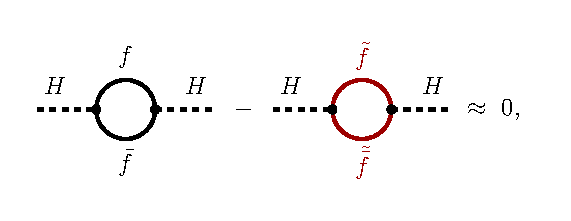
\includegraphics[scale = 0.9]{figures/running_diagrams}
\end{figure}
\noindent
where the sfermions are denoted by a tilde (and highlighted in red). For an example calculation of the MSSM effects in the running couplings we refer for example to the respective exercise in \cite{Hebecker2020}.  \newpage The explicit formulas for the beta functions are given by
\begin{equation}
	\beta_{g_i} = \frac{\dd}{\dd t}g_i = \frac{b_i}{16\pi^2} g_i^3 \quad \text{with} \quad (b_1,b_2,b_3) = \left\{\begin{array}{ll}{(\frac{41}{10}, -\frac{19}{6}, 7)} & {\text {in the SM} } \\ {(\frac{33}{5}, 1, -3)} & {\text {in the MSSM}} \end{array}\right. 
\end{equation}
where $t = \log\frac{Q}{m_Z}$. For $\alpha_i = g_i^2/4\pi$ this yields 
\begin{equation}
	\frac{\dd }{\dd t} \alpha_i^{-1} = -\frac{b_i}{2\pi}.
\end{equation}
As we see in the right plot in Figure \ref{fig:runnings} the unification of the gauge couplings at some high energy scale may be realized in the MSSM. In the end it remains a complicated fine tuning task\footnote{There has been a lot of work considering the qualitative assessment of fine-tuning in theoretical models. Probably the most commonly used measure of fine tuning is the Barbieri-Giudice measure characterized by $\Delta_i \equiv \abs{\frac{\partial \operatorname{ln} m_Z^2}{\partial \operatorname{ln} p_i}}$, where the $p_i$ are the MSSM parameters at the scale $M_X$ which are set by the fundamental SUSY breaking dynamics. The larger the value of $\Delta \equiv \operatorname{max} \Delta_i$ the more fine tuning is needed  \cite{PDG20182019, Hebecker2020}.}. \\
At this point we want to remark that even if this result might look very interesting, and was often referred to as one of the most promising advertisements for the realization of SUSY in nature, it is of course only an approximate result and the picture will already look a lot different at the next loop order.

\begin{figure}[t]
\hfill
	\begin{subfigure}
		\centering
	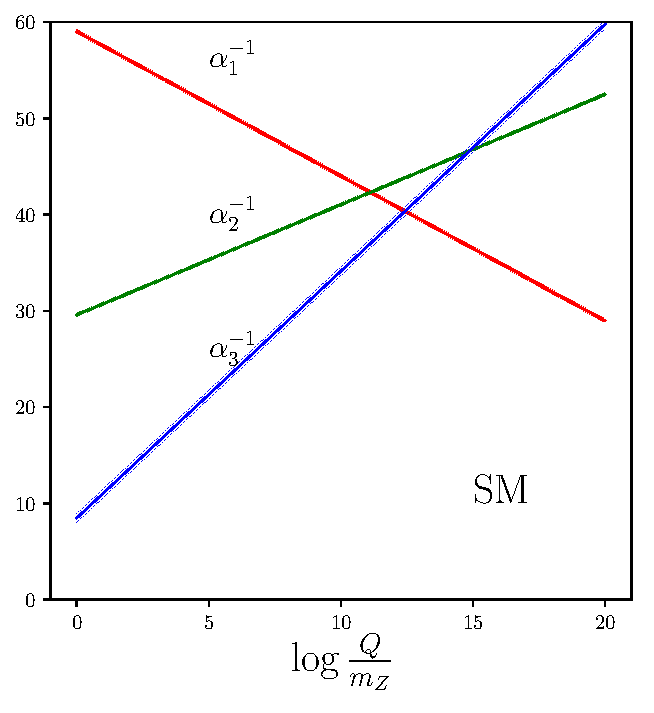
\includegraphics[scale = 0.55]{figures/dgut-1}
	\end{subfigure}
	\hfill
	\begin{subfigure}
		\centering
	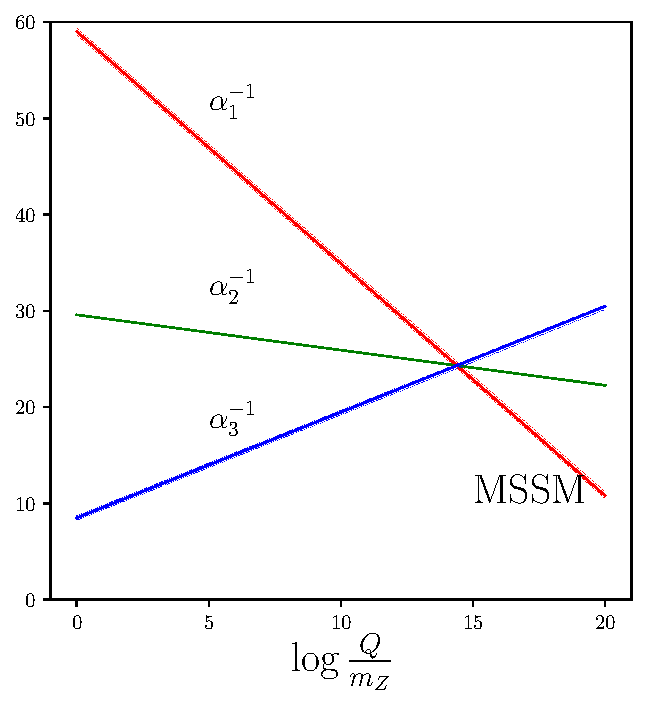
\includegraphics[scale = 0.55]{figures/dgut-2}
	\hfill
	\end{subfigure}
\caption{Running of the (inverse) gauge couplings in the SM and the MSSM, plots inspired by \cite{Kazakov2000}.}
\label{fig:runnings}
\end{figure}







